
%\RequirePackage{pdf15}

\documentclass{beamer}

\usepackage[utf8]{inputenc}

\usepackage{mystyle}
\usepackage{algorithm}
\usepackage[noend]{algorithmic}

\usepackage{tikz}
\usepackage{pgfplots}
\usepackage{subcaption}

%\usepackage{natbib}
\usepackage[style=authortitle,backend=biber]{biblatex}
\addbibresource{anthology.bib}
\addbibresource{emnlp2020.bib}
\renewcommand{\footnotesize}{\scriptsize}

\usepackage{tikz-dependency}
\usetikzlibrary{shapes.arrows, positioning, fit, bayesnet,
    arrows,backgrounds,patterns,matrix,calc,shadows,plotmarks,
    shapes,positioning,automata,positioning,spy,scopes,chains,decorations,decorations.pathreplacing}

\newcommand{\FancyUpArrow}{
\begin{tikzpicture}[baseline=-0.3em]
\node[single arrow,draw,rotate=90,single arrow head extend=0.2em,inner
ysep=0.2em,transform shape,line width=0.05em,top color=green,bottom color=green!50!black] (X){};
\end{tikzpicture}}
\newcommand{\FancyDownArrow}{
\begin{tikzpicture}[baseline=-0.3em]
\node[single arrow,draw,rotate=-90,single arrow head extend=0.2em,inner
ysep=0.2em,transform shape,line width=0.05em,top color=red,bottom color=red!50!black] (X){};
\end{tikzpicture}}

\AtBeginSection[]{
  \begin{frame}
  \vfill
  \centering
  \begin{beamercolorbox}[sep=8pt,center,shadow=true,rounded=true]{title}
    \usebeamerfont{title}\insertsectionhead\par%
  \end{beamercolorbox}
  \vfill
  \end{frame}
}

% quotes
\usepackage[style=british]{csquotes}

\def\signed #1{{\leavevmode\unskip\nobreak\hfil\penalty50\hskip1em
  \hbox{}\nobreak\hfill #1%
  \parfillskip=0pt \finalhyphendemerits=0 \endgraf}}

\newsavebox\mybox
\newenvironment{aquote}[1]
  {\savebox\mybox{#1}\begin{quote}\openautoquote\hspace*{-.7ex}}
  {\unskip\closeautoquote\vspace*{1mm}\signed{\usebox\mybox}\end{quote}}

%Information to be included in the title page:
\title{Low-Rank Factorizations for Fast Inference in Structured Models}
\author{Justin Chiu* \inst{1} \and Yuntian Deng* \inst{2} \and Alexander Rush \inst{1}}
\institute[shortinst]{\inst{1} Cornell Tech \and \inst{2} Harvard University}

\setbeamertemplate{navigation symbols}{} 
\setbeamertemplate{footline}[frame number]

% hypergraph

 
\begin{document}

\begin{frame}[plain]
\titlepage
\end{frame}

\begin{frame}
\frametitle{Structured Models}
\begin{itemize}
\item Explicitly model output associations
\vspace{1em}
    \begin{itemize}
    \item Directly or through latent variables
    \end{itemize}
\vspace{1em}
\item Focus on combinatorially large latent \underline{discrete structures}
\vspace{1em}
    \begin{itemize}
    \item Complementary to continuous, distributed representations
    \end{itemize}
\end{itemize}
\end{frame}

\begin{frame}
\frametitle{Scaling Structured Models}

\begin{itemize}
\item Prior work demonstrated: Size \FancyUpArrow ~ Performance \FancyUpArrow
    \begin{itemize}
    \item Hidden Markov Models (HMM) \footcite{dedieu2019learning,chiu2020hmm}
    \item Probabilistic Context-Free Grammars (PCFG) \footcite{yang2021pcfg}
    \end{itemize}
\vspace{1em}
\item This work: low-rank matrix factorizations
    \begin{itemize}
    \item Generalize to hypergraph models
    \end{itemize}
\end{itemize}
\end{frame}

\begin{frame}
\frametitle{Inference as Matrix-Vector Products}
\begin{itemize}
\item Inference: sequence of matrix-vector products
\vspace{1em}
\item Speed up via fast matvec methods 
\vspace{1em}
\item Applies to a large family of structured models
\end{itemize}
\end{frame}

\begin{frame}
\frametitle{Fast Matrix-Vector Products}
\begin{itemize}
\item Matvecs take $O(L^2)$ computation
\vspace{1em}
\item Various fast methods
    \begin{itemize}
    \item Sparsity (nnz entries)
    \item Fast Fourier Transform ($L \log L$)
    \item \underline{Low-Rank factorization} ($LR$)
    \end{itemize}
\vspace{1em}
\item Connected to efficient attention and kernel approximations
\footcite{performer,rfa,blanc2018adaptive}
\end{itemize}
\end{frame}

\begin{frame}
\frametitle{Roadmap}
\begin{itemize}
\item Inference in HMMs and PCFGs as matvecs
\vspace{1em}
\item Low-rank matvec inference
\vspace{1em}
\item Generalization to hypergraph inference
\vspace{1em}
\item Experiments
\end{itemize}
\end{frame}

\section{Inference as Matvecs}

\begin{frame}
\frametitle{Hidden Markov Models (HMMs)}

For times $t$, model states $z_t \in [L] = \mcL$, and tokens $x_t \in [X] = \mcX$,

\vspace{1em}

\begin{center}
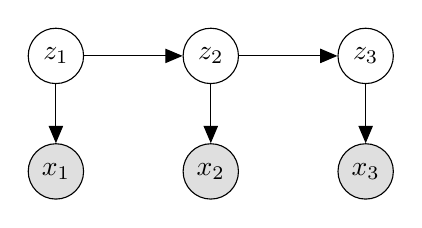
\begin{tikzpicture}[]
\node[latent] (z0) {$z_1$} ;
\node[latent] (z1) [right=1.25cm of z0] {$z_2$} ;
\node[latent] (z2) [right=1.25cm of z1] {$z_3$} ;

\node[obs]    (x0) [below = 0.75cm of z0] {$x_1$};
\node[obs]    (x1) [below = 0.75cm of z1] {$x_2$};
\node[obs]    (x2) [below = 0.75cm of z2] {$x_3$};

\edge {z0} {x0};
\edge {z1} {x1};
\edge {z2} {x2};
\edge {z0} {z1};
\edge {z1} {z2};
\end{tikzpicture}
\end{center}

\vspace{1em}
with joint distribution
$$p(x,z) = \prod_t p(x_t \mid z_t)p(z_t \mid z_{t-1})$$
\end{frame}

\begin{frame}
\frametitle{Inference in HMMs}
Given observed $x = (x_1, \ldots, x_T)$,
\vspace{1em}
we wish to maximize
\begin{equation*}
p(x)
= \sum_{z_1}\cdots\sum_{z_T}p(x, z)
= \bm1^\top\Psi_1\Psi_2\cdots\Psi_T\bm1,
\end{equation*}
where
\begin{align*}
[\Psi_{t}]_{z_t,z_{t+1}} &= p(z_{t+1},x_t \mid z_t)\\
[\Psi_{1}]_{z_1,z_2} &= p(z_2,x_1 \mid z_1)p(z_1)
\end{align*}
\end{frame}

\begin{frame}
\frametitle{Matvec Inference in HMMs}

\begin{algorithm}[H]
\caption{HMM Inference}
\begin{algorithmic}
\FOR {$t \leftarrow (t+1)$ in right-to-left order}
%\FOR {$z_{t+1} \in \mcL$}
%\STATE $[\beta_{t+1}]_{z_{t+1}} = [\alpha_{t+1}]_{z_{t+1}}$
%\ENDFOR
%\STATE $\alpha_t \stackrel{+}{\gets} \Psi_t \beta_{t+1}$
\STATE $\beta_t \stackrel{+}{\gets} \Psi_t \beta_{t+1}$
\ENDFOR
%\STATE \textbf{return} $\alpha_0^\top \mathbf{1}$
\STATE \textbf{return} $\beta_0^\top \mathbf{1}$
\end{algorithmic}
\end{algorithm}
\end{frame}

\begin{frame}
\frametitle{Probabilistic Context-Free Grammars (PCFG)}
A context-free grammar $\mcG = (\mcL,\mcR)$ where
$$
    \mcL: \text{ Node labels};\qquad
    \mcX: \text{ Tokens};\qquad
    \mcR: \text{ Rules},
$$
where rules take the form
\begin{align*}
A&\to B\ C, & A,B,C\in\mcL \\
P&\to x, & P \in\mcL,x\in\mcX
\end{align*}

In a PCFG, each rule has probability mass
$$p(r) = p(B,C \mid A)$$
The joint distribution over rules in a tree $t$
$$p(t) = \prod_{r\in t} p(r)$$

\end{frame}

\begin{frame}
\frametitle{Inference in PCFGs}

\begin{itemize}
\item For a given observation $x$, compute $p(x) = \sum_{t: \text{yield}(t) = x} p(t)$
via dynamic programming
\vspace{1em}
\item For each span $(i,k)$, sum over split point $j \in (i,k)$:

\begin{center}
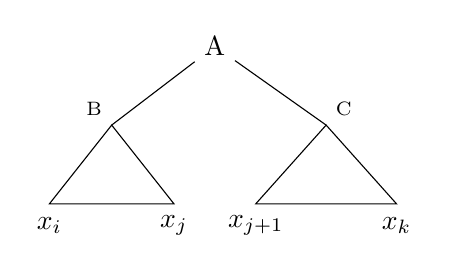
\begin{tikzpicture}
\node (a) [minimum height = 1.5em] {$x_i$};
\node (b) [right=of a, minimum height = 1.5em] {$x_j$};
\node (b2) [right=.75em of b, minimum height = 1.5em] {$x_{j+1}$};
\node (c) [right=of b2, minimum height = 1.5em] {$x_k$};

\coordinate (bbx) at ($ (b.north) + (b2.north) $);

\node (d) at ($ 0.5*(bbx) + (0,2) $) {A};

\coordinate (abx) at ($ (a.north) + (b.north) $);
\coordinate [label=above left:{B}] (ab) at ($ 0.5*(abx) + (0,1) $);
\draw (a.north) -- (b.north) -- (ab) -- cycle;

\coordinate (bcx) at ($ (b2.north) + (c.north) $);
\coordinate [label=above right:{C}] (bc) at ($ 0.5*(bcx) + (0,1) $);
\draw (b2.north) -- (c.north) -- (bc) -- cycle;

\draw (ab) -- (d);
\draw (bc) -- (d);

\end{tikzpicture}
\end{center}

\item Similar to HMMs, define
$$[\Psi]_{z_u, (z_1,z_2)} = p(B=z_1,C=z_2 \mid A=z_u),$$
for each rule

\end{itemize}

\end{frame}

\begin{frame}
\frametitle{Matvec Inference in PCFGs}


\begin{algorithm}[H]
\caption{PCFG Inference}
%\small
\begin{algorithmic} 
\FOR {$(i,k) \leftarrow (i,j), (j,k)$ in span-size order}
\FOR {$z_1,z_2 \in \mcL_{i,j}\times\mcL_{j,k}$}
\STATE $[\beta_{i,j,k}]_{(z_1,z_2)} = [\alpha_{i,j}]_{z_1}[\alpha_{j,k}]_{z_2}$
\ENDFOR
\STATE $\alpha_{i,k} \stackrel{+}{\gets} \Psi_{i,j,k}\beta_{i,j,k}$
\ENDFOR
\STATE \textbf{return} $\alpha_{1,T}^\top \mathbf{1}$
\end{algorithmic}

\end{algorithm}
\end{frame}

\section{Speeding Up Inference}

\begin{frame}
\frametitle{Low-Rank Factorization}
\begin{itemize}
\item Factor matrices $\Psi=UV^\top$,
$U\in\R^{L \times R},V\in\R^{L'\times R}$
\[
\vcenter{\hbox{\begin{tikzpicture}[baseline=-0.5ex]
    \draw (0,0) rectangle (2,1.5) node[pos=.5] {$\Psi$};
\end{tikzpicture}}}
\times
\vcenter{\hbox{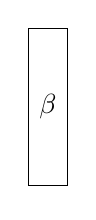
\begin{tikzpicture}[baseline=-0.5ex]
    \draw (0,0) rectangle (.5,2) node[pos=.5] {$\beta$};
\end{tikzpicture}}}
=
\vcenter{\hbox{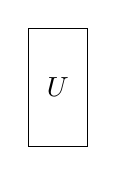
\begin{tikzpicture}[baseline=-0.5ex]
    \draw (0,0) rectangle (.75,1.5) node[pos=.5] {$U$};
\end{tikzpicture}}}
\times
\left(\,
\vcenter{\hbox{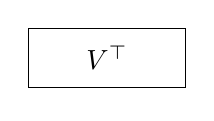
\begin{tikzpicture}[baseline=-0.5ex]
    \draw (0,0) rectangle (2,.75) node[pos=.5] {$V^\top$};
\end{tikzpicture}}}
\times
\vcenter{\hbox{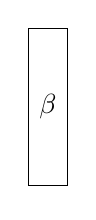
\begin{tikzpicture}[baseline=-0.5ex]
    \draw (0,0) rectangle (.5,2) node[pos=.5] {$\beta$};
\end{tikzpicture}}}
\,\right)
\]
\item Two matrix-vector products of cost $O(LR)$ and $O(L'R)$
\end{itemize}
\end{frame}

\begin{frame}
\frametitle{Expressiveness and Generality}
\begin{itemize}
\item Rank constraints limit expressivity
\vspace{1em}
\item Only apply to a subset of parameters
    \begin{itemize}
    \item Transition matrix for HMMs
    \item Subset of the transition matrix for PCFGs
    \end{itemize}
\vspace{1em}
\item Is it more expressive than a smaller model?
    \begin{itemize}
    \item An $L$-state HMM with rank $R$ $(< L)$ is more
        expressive than an $R$-state HMM
    \end{itemize}
\vspace{1em}
\item What other models does this work for?
    \begin{itemize}
    \item Hypergraph models!
    \end{itemize}
\end{itemize}
\end{frame}

\begin{frame}
\frametitle{Hypergraph Marginalization}
\begin{itemize}
\item Models where exact inference is a directed acyclic hypergraph
\vspace{1em}
\item Hypergraph contains a node set and hyperedge set
    \begin{itemize}
    \item Nodes have label set $\mcL$
    \item Hyperedges join a single head node $u$ and a list of tail nodes $v$
    \end{itemize}
\end{itemize}

\vspace{1em}

\begin{columns}

\begin{column}{0.5\textwidth}
\begin{center}
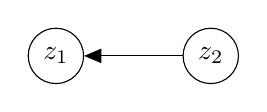
\begin{tikzpicture}[]
\node[latent] (z0) {$z_1$} ;
\node[latent] (z1) [right=1.25cm of z0] {$z_2$} ;

\edge {z1} {z0};
\end{tikzpicture}
\end{center}
\end{column}

\begin{column}{0.5\textwidth}
\begin{center}
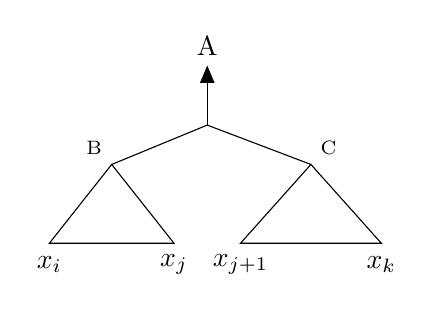
\begin{tikzpicture}
\node (a) [minimum height = 1.5em] {$x_i$};
\node (b) [right=of a, minimum height = 1.5em] {$x_j$};
\node (b2) [right=.2em of b, minimum height = 1.5em] {$x_{j+1}$};
\node (c) [right=of b2, minimum height = 1.5em] {$x_k$};
\coordinate (bbx) at ($ (b.north) + (b2.north) $);

\coordinate (abx) at ($ (a.north) + (b.north) $);
\coordinate [label=above left:{B}] (ab) at ($ 0.5*(abx) + (0,1) $);
\draw (a.north) -- (b.north) -- (ab) -- cycle;
\coordinate (bcx) at ($ (b2.north) + (c.north) $);
\coordinate [label=above right:{C}] (bc) at ($ 0.5*(bcx) + (0,1) $);
\draw (b2.north) -- (c.north) -- (bc) -- cycle;

\coordinate (abc) at ($ 0.5*(bbx) + (0,1.5) $);
\node (d) at ($ 0.5*(bbx) + (0,2.5) $) {A};

\draw (ab) -- (abc);
\draw (bc) -- (abc);
\draw [->] (abc) -- (d);

\end{tikzpicture}
\end{center}
\end{column}

\end{columns}

\begin{center}
Hyperedge representations for HMMs and PCFGs
\end{center}

\end{frame}

\begin{frame}
\frametitle{Hypergraph Marginalization Algorithms}
\centering
\begin{algorithm}[H]
%\hspace{.5em}
%\begin{algorithm}[H]
\caption{\label{alg:hypergraph-marg} Hypergraph marginalization}
\begin{algorithmic} 
\FOR {$u \leftarrow v$ hyperedge $e$ topologically}
\STATE $\beta_v \gets \alpha_{v_1}\alpha_{v_2}^\top$
    \hfill $\vartriangleright$ $O(L^{|e|})$
\STATE $\alpha_u \stackrel{+}{\gets} \Psi_e\beta_v$
    \hfill $\vartriangleright$ $O(L^{|e|+1})$
\ENDFOR
\STATE \textbf{return} $\alpha_S^\top \mathbf{1}$
\end{algorithmic}

%\end{algorithm}
\end{algorithm}

\begin{algorithm}[H]
%\begin{comment}
\caption{\label{alg:low-rank-update} Low-rank marginalization}
\begin{algorithmic} 
\FOR {$u \leftarrow v_1, v_2$ hyperedge $e$ topologically}
\STATE $\beta_v \gets \alpha_{v_1}\alpha_{v_2}^\top$
    \hfill $\vartriangleright$ $O(L^{|e|})$
\STATE $\gamma \gets V_e^\top\beta_v$
    \hfill $\vartriangleright$ $O(L^{|e|}R)$
\STATE $\alpha_u \stackrel{+}{\gets} U_e\gamma $
    \hfill $\vartriangleright$ $O(LR)$
\ENDFOR
\STATE \textbf{return} $\alpha_S^\top\mathbf{1}$
\end{algorithmic} 
\end{algorithm}

\end{frame}


\section{Experiments}

\begin{frame}
\frametitle{Experiments}
\begin{itemize}
\item Compare speed vs accuracy frontier
\vspace{2em}
\item Language modeling on \textsc{Penn Treebank} \footcite{ptb}
    \vspace{1em}
    \begin{itemize}
    \item Softmax HMM and PCFG vs low-rank versions (LHMM, LPCFG)
    \item Evaluate accuracy with perplexity, a function of likelihood
    \end{itemize}
\vspace{2em}
\item Video modeling on \textsc{CrossTask} \footcite{zhukov2019cross}
    \vspace{1em}
    \begin{itemize}
    \item Softmax HSMM vs low-rank HSMM
    \item Evaluate accuracy with negative log-likelihood
    \end{itemize}
\end{itemize}
\end{frame}

\begin{frame}
\frametitle{HMM Speed vs Accuracy}
\centering
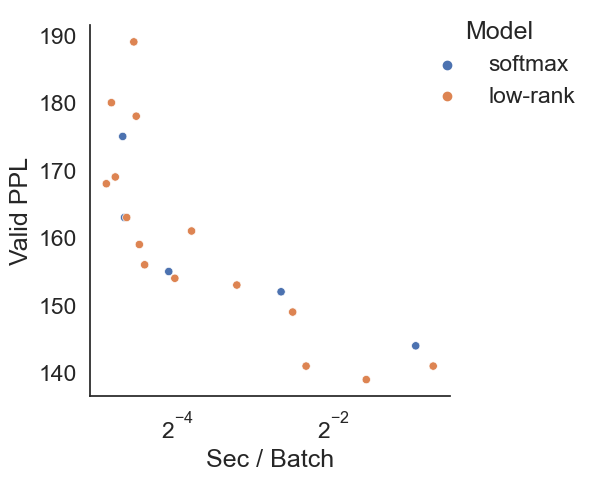
\includegraphics[height=3in]{imgs/hmm/lhmm-speed-accuracy.png}
\end{frame}

\begin{frame}
\frametitle{PCFG Speed vs Accuracy}
\centering
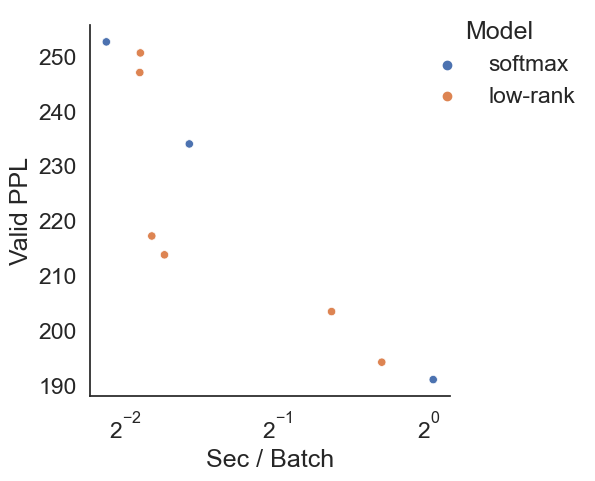
\includegraphics[height=3in]{imgs/hmm/pcfg-speed-accuracy.png}
\end{frame}

\begin{frame}
\frametitle{HSMM Speed vs Accuracy}
\centering
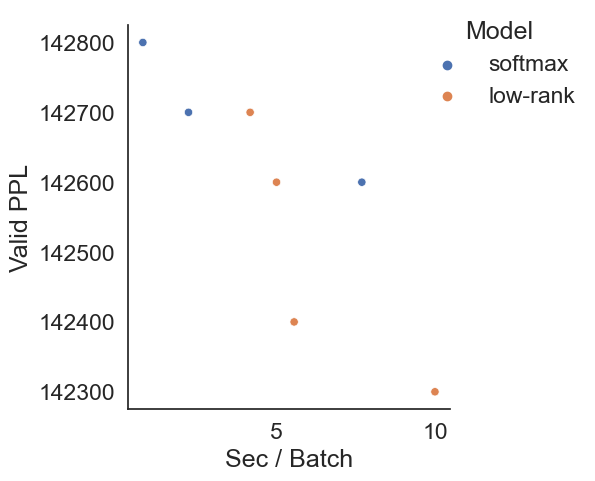
\includegraphics[height=3in]{imgs/hmm/hsmm-speed-accuracy.png}
\end{frame}

\begin{frame}
\frametitle{Conclusion}
\begin{itemize}
\item Introduce a low-rank factorization to speed up inference
\vspace{2em}
\item Applies to models with hypergraph inference
\vspace{2em}
\item Most effective with large models
\end{itemize}
\end{frame}


\begin{frame}[allowframebreaks]
\frametitle{Citations}
\printbibliography
\end{frame}


\begin{frame}
\frametitle{HMM Music Results}
\centering
\begin{tabular}{lrrrr}
\toprule
Model       & Nott & Piano & Muse & JSB \\
\midrule
%RNN      & 4.46       & 8.37        & 8.13       & 8.71          \\ 
%\midrule 
RNN-NADE & 2.31  & \textbf{7.05}        & \textbf{5.6}        & 5.19          \\
%\midrule
R-Transformer & \textbf{2.24} & 7.44 & 7.00 & 8.26 \\
LSTM  & 3.43 & 7.77   & 7.23 & 8.17     \\
%\midrule
LV-RNN    & 2.72       & 7.61        & 6.89       &\textbf{ 3.99}\\
SRNN     & 2.94       & 8.20         & 6.28       & 4.74          \\
\midrule
TSBN     & 3.67       & 7.89        & 6.81       & 7.48          \\
HMM &  2.43 & 8.51 & 7.34 & 5.74 \\
LHMM & 2.60 & 8.89 & 7.60 & 5.80 \\
\bottomrule
\end{tabular}
\end{frame}

\begin{frame}
\frametitle{PCFG Results}

\begin{center}
\begin{tabular} {lllrrrr}
\toprule
$|\mathcal{N}|$ & $|\mathcal{P}|$ & Model & $N$ &  PPL & Batch/s\\
\midrule
30  & 60    & PCFG & - & 252.60 & 4.37\\
    &       & LPCFG & 8 &  247.02    & 3.75\\
    &       & LPCFG & 16 & 250.59    & 3.74\\
\midrule
60  & 120   & PCFG & - & 234.01 & 2.99\\
    &       & LPCFG & 16& 217.24 & 3.55\\
    &       & LPCFG & 32& 213.81 & 3.35\\
\midrule
100 & 200   & PCFG & - &  191.08   & 0.98\\
    &       & LPCFG & 32& 203.47 & 1.56\\
    &       & LPCFG & 64& 194.25 & 1.24\\
\bottomrule
\end{tabular}
\end{center}
\end{frame}

\begin{frame}
\frametitle{HSMM Results}
\begin{center}
\begin{tabular} {lllrrrr}
\toprule
Model & $L$ & $N$ & NLL & Batch/s \\
\midrule
HSMM & $2^6$ & - & $1.428e5$ & 1.28 \\
HSMM & $2^7$ & - & $1.427e5$  & 0.45\\
HSMM & $2^8$ & - & $1.426e5$ & 0.13 \\
\midrule
LHSMM & $2^7$ & $2^7$ & $1.427e5$ & 0.24 \\
LHSMM & $2^8$ & $2^6$ & $1.426e5$ & 0.20 \\
LHSMM & $2^9$ & $2^5$ & $1.424e5$ & 0.18 \\
LHSMM & $2^{10}$ & $2^4$ & $1.423e5$ & 0.10 \\
\bottomrule
\end{tabular}
\end{center}
\end{frame}

\end{document}
